%%%
% How the results given can be of use to a future project
% despite shortcomings
%%%

\subsection{Usefulness of Results}

%%%
% Intro paragraph
%%%

%%%
Despite the final learned agent's shortcomings in ability to consistently win
a single game,
the deliverables of this project can still be applied to expand the current
knowledge of cribbage as well as serve as a guidance story.
%
As they were intended from the outset,
the generated strategy graphs can serve as a set of guidelines as to how a
player ``should'' be playing a certain hand.
%
Although a human player may not be able to calculate the statistics which the
agent used as accurately as a computer,
a fair amount of experience and intuition can be gained through repeated
play which should approximate the expected and guaranteed returns well.
%%%

%%%
The agent's successes in the macro scale can also be of use to those
applications which also operate on the scale of thousands to millions of games.
%
Mainly,
the developed agent could be used for a first round or two of training
of a value-function based agent.
%
Rather than learning from the self-play with no existing knowledge,
a policy-following agent can be played against instead.
%
Playing an agent of greater difficulty would allow the value function optimizing
agent to more quickly converge to an optimum.
%
Since the results of this thesis were achieved without imparting any particular 
pre-existing domain knowledge to the initial policy,
this faster convergence to optimal would not be unfairly biased
towards any form of human play,
thus lowering training time without introducing suboptimalities.
%%%


% Figures

\begin{figure}
\center
\begin{subfigure}[b]{0.66\textwidth}
	\center
	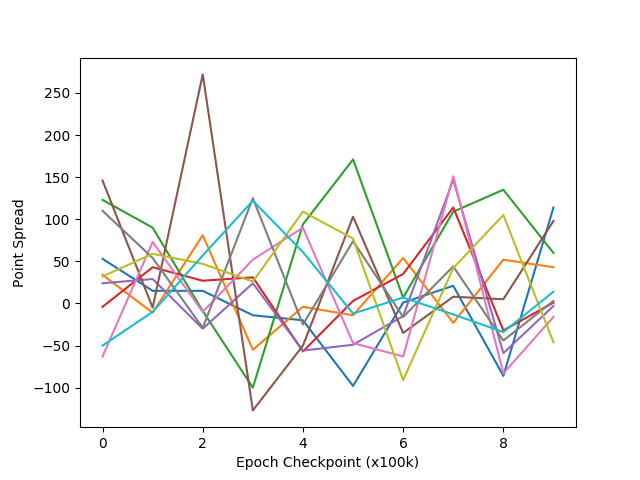
\includegraphics[height=0.22\textheight]{images/discussion/usefulness/r2-time-series-9.png}
	\caption{Point spreads for 9-game matches, like in human play.}
	\label{r2-time-series-9}
\end{subfigure}
~
\begin{subfigure}[b]{0.66\textwidth}
	\center
	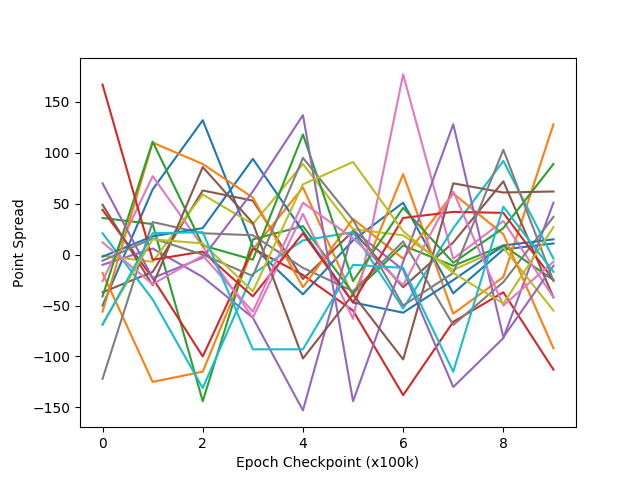
\includegraphics[height=0.22\textheight]{images/discussion/usefulness/r2-time-series-100.png}
	\caption{Point spreads for 100-game matches.}
	\label{r2-time-series-100}
	% TODO: ^^^ make sure we have an accurate graph,
	%		scale leads me to believe we have the wrong graph
\end{subfigure}

\begin{subfigure}[b]{0.66\textwidth}
	\center
	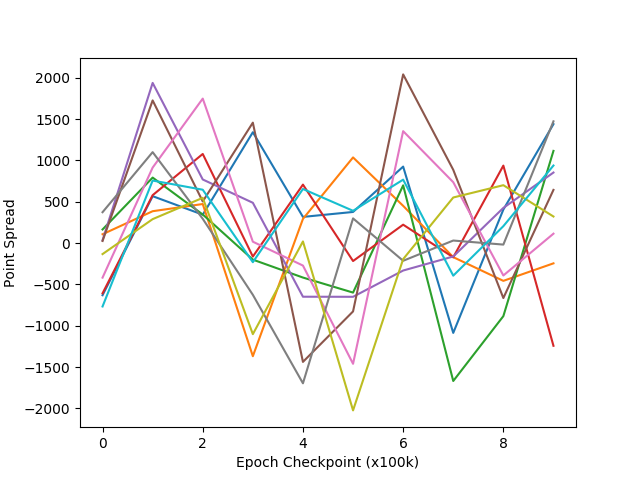
\includegraphics[height=0.22\textheight]{images/discussion/usefulness/r2-time-series-1000.png}
	\caption{Point spreads for 1,000-game matches.}
	\label{r2-time-series-1000}
\end{subfigure}
~
\begin{subfigure}[b]{0.66\textwidth}
	\center
	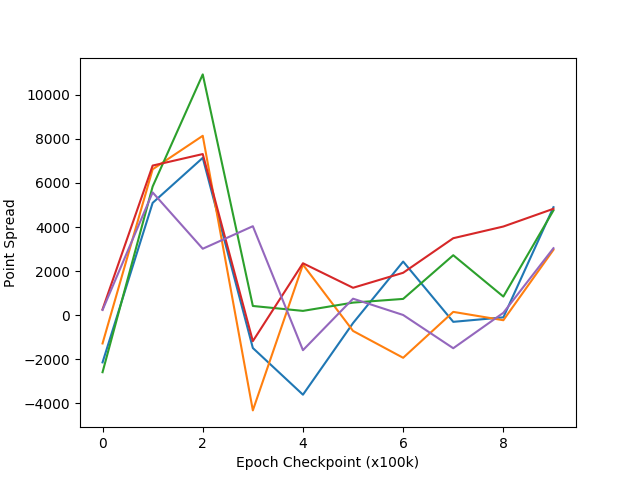
\includegraphics[height=0.22\textheight]{images/discussion/usefulness/r2-time-series-10000.png}
	\caption{Point spreads for 10,000-game matches.}
	\label{r2-time-series-10000}
\end{subfigure}

\caption{
	Point spreads across matches of varying lengths.
	In each graph,
	the final \learned\ agent is played against its previous checkpoint
	iterations.
}
\label{fig:r2-time-series}
\end{figure}

% /Figures


%%%
% Discussion of how scale affects score spreads
%	On 9-game scale, we have utter chaos, maybe not worth mentioning?
%	On 100-game scale, utter chaos
%	On 1000-game scale, maybe a little, if we squint hard,
%	On 10k-game scale, we can see a pattern
%		contradicts the 1k-game observations
%		consistently even with random
%		sharp increase in performance over 100k-200k
%		even play for the next 600k
%		seemingly regain advantage in the last 200k
%%%

%%%
A regulation cribbage match between two human players consists of nine games.
%
As can be seen in Figure~\ref{fig:r2-time-series-100},
in a series of 100-game matches between a fully trained agent and its
previous checkpoints,
no pattern is discernible in total point spreads between the two playing agents.
%
This demonstrates that,
on this scale,
the winner of the game is no more predictable than a truly random coin toss.
%%%

%%%
When the scale is increased to one thousand games,
a slight pattern begins to emerge
when visualized in Figure~\ref{fig:r2-time-series-1000}
%
Whereas the majority of the graph remains highly varying and unpatterned,
the first few games follow a common pattern.
%
The match against the random agent is still unpredictable,
but the matches against the 100,000 and 200,000 game trained checkpoints are
consistently beaten by the final agent.
%%%

%%%
Although fewer matches are played to accommodate the increased time needed to
play the increased number of games,
the same pattern present in the thousand-game scale is visible in the
ten thousand-game matches.
%
With the exception of the purely untrained agent,
the least \learned\ agents perform the poorest against the final
\learned\ agent.
%
Play are approximately evenly matched when between agents
when the opposing agent has trained for 300,000 to 700,000 games.
%
Following these matches,
the agent begins to again win more consistently when more training is done.
%%%

%%%
If the agent is being trained correctly and no overfitting is occurring,
then the point spread should be a positive number,
gradually decreasing and approaching zero
as more training is applied to its opponent,
forming a similar curve to a loss metric used in classical machine learning.
%
In the event of overfitting,
the curve would dip below the zero before reapproaching zero.
%
Neither of these shapes were seen in the resulting graph
(see Figure~\ref{r2-time-series-10000}).
%
Instead,
the shape of the curve implies that,
since the random agent performs consistently better than the trained agent,
the learning process is not learning the game so much as how to outplay its
opponent.
%
This conclusion is supported by the observation that the agents with limited
training are steadfastly outplayed.
%%%

%%%
However,
since there is a sharp dip after 300,000 training epochs before increasing
again,
the results are difficult to interpret.
%
The final \learned\ agent is more evenly matched in performance with an agent
trained for 400,000 games
than it is against a more recently trained agent.
%
The reintroduction of an increasing curve
is an indicator of overfitting in the middle stages.
%
Whereas the final agent is able to play well against these agents,
they themselves have decreased in performance capability.
%
This is speculated to be a result of learning how to outplay its opposing agent
rather than an understanding of the game.
%
This is contingent upon the results of the round-robin play though,
so no conclusions can be drawn at this time.
% TODO ^^^ reaffirm when round-robin play is completed
%%%

%%%
Also of further note is the scale on the aforementioned graphs.
%
In Figure~\ref{r2-time-series-10000},
the maximum point spread achieved is just a shade above 10,000 points
over the course of 10,000 games.
%
This means that the average point spread advantage is approximately 
one point per game at peak performance\textemdash
and most often $0.2$ points per game\textemdash
in long-term play.
%
The average spread increases to $25$ points per game when fewer games are 
played,
but since performance is unpredictable on this scale,
this can be explained as a result of the randomness of the cards given
and cannot be considered a reliable measure of performance.
%
In fact,
in sampled matches,
it was not uncommon to observe losses and wins of 30 points or more
as well as much closer games with margins of only a few points.
%
In addition to the randomness of cards dealt,
this massive point sway could also be the result of the agents' uncertainty on 
how to recover from a losing position.
%
While the reasons for this inability cannot be said to be more than speculation,
the learning of a policy directly without taking into account cards dealt
is the likely culprit,
as explained previously.
%%%



%\input{sections/discussion/usefulness/*}
